\documentclass[12pt]{article}
\usepackage[a4paper, margin=1in]{geometry}
\usepackage{graphicx}
\usepackage{amsmath}
\usepackage{hyperref}
\usepackage{titlesec}
\usepackage{setspace}
\usepackage{enumitem}
\usepackage{natbib}
\usepackage{tikz}
\usepackage{amssymb}
\usepackage{float}
\usetikzlibrary{trees}
\titleformat{\section}{\normalfont\Large\bfseries}{\thesection.}{1em}{}
\titleformat{\subsection}{\normalfont\large\bfseries}{\thesubsection.}{1em}{}

\title{Network Games and Agricultural Collectivization in China}
\author{Xinkai Xu, Liming Lin, Zihao Liu}
\date{\today}

\begin{document}

\maketitle
\onehalfspacing

\begin{abstract}
This project uses the framework of network games to analyze incentive structures and behavioral dynamics in the context of Chinese agricultural collectivization during the 1960s and 1970s. Starting from a baseline model of small reciprocal production teams, we incrementally build up to more complex systems. Firstly, we expand the network by conecting different teams, allowing for inter-team interactions. Then we add signaling games to capture the information assymetries and communications among agents. Finally, we introduce external shocks to the system, such as natural disaster, to study the reactions of different network structures. And we find that ...
\end{abstract}

\section{Introduction}

Agricultural collectivization has been one of the most prominent and controversial policies in modern China. Existing studies (\cite{chinnDiligenceLazinessChinese1980, nitzanDiligenceLazinessChinese1987}) have used game-theoretic approaches such as the Prisoner’s Dilemma to model individual incentives and effort in collective settings. While insightful, these models often assume homogeneity and lack the structural complexity seen in real-world rural networks and governance.\\

This project expands the analytical lens by incorporating \textbf{network games} to capture how local interdependencies shape collective effort and participation decisions. Households in a commune do not interact uniformly; instead, their decisions are influenced by their neighbors' behavior, visibility, and reputational spillovers. Network games offer a natural framework to reflect this decentralized but interconnected structure.\\

Furthermore, to analyze the vertical interactions between local commune leaders and higher-level government officials—especially under asymmetric information and crisis conditions—we introduce \textbf{signaling games}. During natural disasters or in the context of procurement targets, local leaders often faced incentives to misreport productivity or overstate effort to secure promotions or avoid sanctions. Signaling games allow us to formally represent these strategic misalignments and the role of beliefs and incentives in shaping observed actions.\\

By combining network and signaling models, we aim to offer a richer, more institutionally grounded understanding of how collectivization outcomes emerged—not just from household-level decisions, but also from the complex interplay between local coordination and hierarchical governance.\\

\section{Base Model: The Small Network within a Commune}
Let $I = \{1, 2, \dots, n\}$ denote the set of players, $n > 1$, connected by a network $G$. We use matrix $G$ to track the connections in this network. We define $g_{ij} = 1=g_{ji}$ if $i$ and $j$ are linked to each other, and $g_{ij} = 0$ otherwise.  We also set $g_{ii} = 0$. The neighborhood of the individual $i$ is the set given by $[ N_i := j \mid g_{ij}] = 1$. Therefore, $|N_i|$, the cardinality, which is $\sum_j g_{ij}$, is called the \textbf{degree} of $i$.\\

We use the following quadratic utility function to capture the \emph{strategy complementarity}:
\[
U_i(x_i, x_{-i}, G_i) = \alpha x_i - \frac{1}{2} x_i^2 + \beta x_i \sum_j g_{ij} x_j,
\]
where $\alpha$ is the marginal return to effort $x_i$, and $\beta$ is the strength of strategic interactions.

We assume $\beta > 0$, so that we have
\[
\frac{\partial^2 U_i(x_i, x_{-i}, G_i)}{\partial x_i \partial x_j} = \beta g_{ij} > 0,
\]
which reflects strategic complementarity in efforts.

In small groups with $n$ players in a network, people know each other well, and it is reasonable to assume network $G$ is a \textbf{complete network} and players have full information.

\begin{figure}[H]
  \centering
  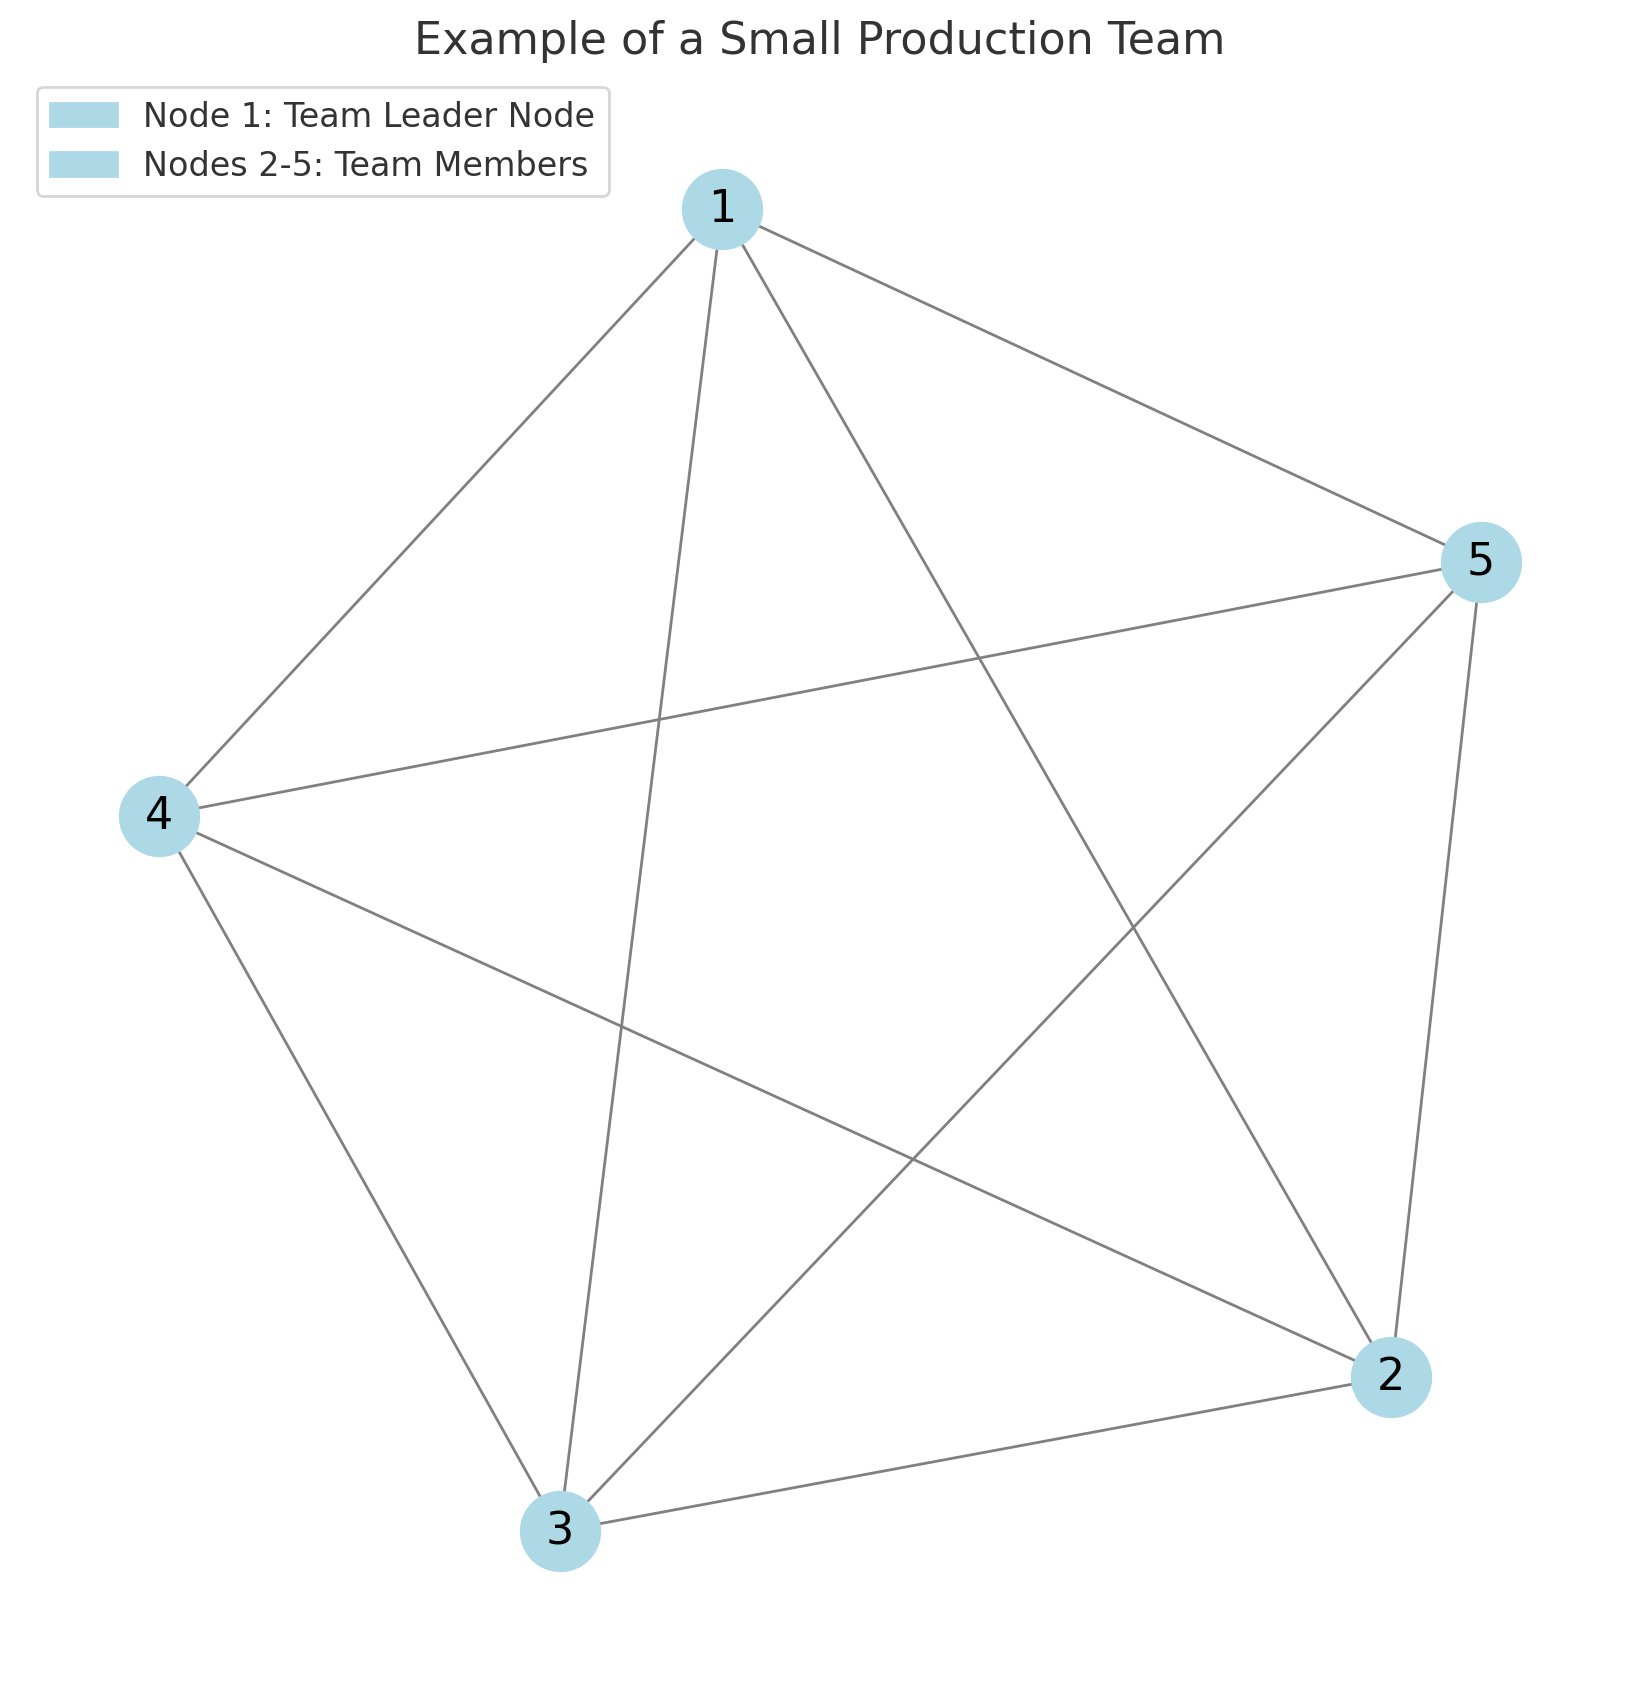
\includegraphics[height=0.6\textwidth]{small network1.png}
  \caption{Example of a Small Production Team}
  \label{fig:small-team}
\end{figure}

In equilibrium, each agent maximizes their utility. By the FOC, we get:
\[
x_i^* = \alpha + \beta \sum_j g_{ij}x_i x_j. \tag{2}
\]

Since $G$ is a complete network, everyone has the same degree. We assume total effort is  
\[
\bar{x} = \sum_i x_i,
\]
and so:
\[
x_i^* = \alpha + \beta \left( \sum_{j \neq i} x_j^* \right) = \alpha + \beta(n - 1)\bar{x}. \tag{3}
\]

Assuming symmetry, i.e., $x_i^* = \bar{x}$ for all $i$, we get:
\[
x_i^* = \frac{\alpha}{1 - \beta(n - 1)}.
\]

Then, in a small group, the utility of agent $i$' is given by:
\[
\frac{\alpha^2}{\beta + 1 - n\beta} - \frac{1}{2} \left( \frac{\alpha}{(\beta + 1 - n\beta)} \right)^2 + \beta(n - 1) \left( \frac{\alpha}{\beta + 1 - n\beta} \right)^2. \tag{4}
\]


\section{Large Networks}
\subsection{Large Network with Without Signaling}
Now we move to the large network setting where there are multiple small groups. And in each small complete network, there is one node that represents the leader of the small group. Between the small groups, there are indirect connections among the small group leaders through a central node the represents higher level government.\\
By this construction, we have three types of players with different degrees.  
We assume $N = nk + 1$, where $n$ is the number of players in a small group, $k$ is the number of small groups.

\begin{itemize}
    \item Type 1: $(n-1)$ degrees (internal to small group)
    \item Type 2: $k$ degrees (one connection to each small group leader)
    \item Type 3: $n$ degrees (small group leader)
\end{itemize}

Incomplete information about $\beta$ without signals.

We assume $\beta$ takes two possible values: $\beta = \{\beta_l,\beta_h\}$ where $\beta_l < \beta_h$. 

We assume each agent holds a belief for $\beta$.

They share a common prior:

\[
\mathbb{P}(\beta = \beta_l) = p, \quad \mathbb{P}(\beta = \beta_h) = 1-p
\]

Therefore we assume there is no communication between players, and the network does not affect the value of $p$.

Then:

\[
\mathbb{E}[x_i] = \alpha - \sum_{j} g_{ij} \mathbb{E}[x_j] + \mathbb{E}[\beta] p_i
\]

where:

\[
\mathbb{E}[\beta] = p \beta_l + (1-p) \beta_h
\]

Also:

\[
\mathbb{E}[x_i] = x_i
\]

Thus:

\[
\alpha - x_i + \mathbb{E}[\beta] p_i - \sum_{j} g_{ij} x_j = 0
\]

\vspace{1em}

Thus:

\[
x_i^* = \alpha + \mathbb{E}[\beta] + \sum_{j=1}^{n} g_{ij} x_j
\]

where $G$ is the network matrix.

\vspace{1em}

The solution is given by:

\[
x^* = \alpha (I_n - \mathbb{E}[\beta] G)^{-1} \mathbf{1}
\]

where $I_n$ is the $n \times n$ identity matrix.

$G$ is the same network matrix as before.

\vspace{1em}

We assume that:

\[
\mathbb{E}[\beta] \leq \frac{1}{\lambda_{\text{max}}(G)}
\]

where $\lambda_{\text{max}}(G)$ is the largest eigenvalue of the network $G$.

\vspace{1em}

Moreover:

\[
(I_n - \mathbb{E}[\beta] p G)^{-1} = P_G \left( I - \mathbb{E}[\beta] p D_G \right)^{-1} P_G^{-1}
\]

where:

\[
G = P_G D_G P_G^{-1}
\]

and $D_G$ is the diagonal matrix of eigenvalues of $G$:

\[
D_G = 
\begin{pmatrix}
\lambda_1 & 0 & \cdots & 0 \\
0 & \lambda_2 & \cdots & 0 \\
\vdots & \vdots & \ddots & \vdots \\
0 & 0 & \cdots & \lambda_n
\end{pmatrix}
\]

\subsection{Large Network with Signaling}
We move to a large network setting where each household only knows its own number of neighbors (degree) and forms beliefs over others' behavior. The model assumes strategic complements or substitutes depending on the distribution mechanism and social context.

There are $M \gg n$ players now. In this case, we treat $\beta$ as important information to capture the feature that in large groups, an agent does not know their neighbors' neighborhoods well.  
This uncertainty introduces people's incomplete information about $\beta$.

We assume that $\beta$ can only take two values, $\beta_L$ or $\beta_H$.  
All individuals share a common prior:
\[
\Pr(\beta = \beta_H) = p, \quad p \in (0,1)
\]

Individuals receive two signals which are not always correct.  
We define:
\[
\Pr(s_i = 1 \mid \beta = \beta_H) = q_1, \quad \Pr(s_i = 1 \mid \beta = \beta_L) = q_2
\]
where $s_i = 1$ and $s_i = -1$ denote the event that agent $i$ has received signal $1$ and $-1$, respectively.

Besides, we assume that the network is no longer a complete network.  
It is given by a graph


The idea is that a large network is composed of several small complete networks.  
And in each small complete network, there is one person who connects with leaders of the large group.

There are three types of players with different degrees.  
We assume $N = nk + 1$, where $n$ is the number of players in a small group, $k$ is the number of small groups.

\begin{itemize}
    \item Type 1: $(n-1)$ degrees (internal to small group)
    \item Type 2: $k$ degrees (one connection to each small group leader)
    \item Type 3: $n$ degrees (small group leader)
\end{itemize}

The utility function is the same for three types of players, given by:

\[
u_i(x_i, x_{-i}) = \alpha_i x_i - \frac{1}{2}x_i^2 + x_i\left( \sum_j g_{ij} x_j \right)
\]

By the first order condition, we get:
\[
x_i = \alpha_i + \sum_j g_{ij} x_j
\]

We define:
\[
b(\beta) = (I - G)^{-1} \alpha(\beta)
\]
where $G$ is the network adjacency matrix and $\alpha(\beta)$ is the $n \times 1$ vector of $\alpha_i$.

When agent $i$ receives signal $s_i = l$, his utility function satisfies:
\[
\mathbb{E}[u_i(x_i, x_{-i}) \mid s_i = l] = \alpha_i(l) x_i - \frac{1}{2}x_i^2 + x_i \left( \sum_j g_{ij} \mathbb{E}[x_j \mid s_i = l] \right)
\]

Thus:
\[
x_i = \alpha_i(l) + \sum_j g_{ij} \mathbb{E}[x_j \mid s_i = l]
\]

By the first order condition on $x_i(l)$, we get:
\[
x_i(l) = \alpha_i(l) + \sum_j g_{ij} \mathbb{E}[x_j(l)]
\]

When agent $i$ receives signal $s_i \in \{L\}$, for each possible $j$ we have:

\[
\mathbb{E}(\beta_j \mid s_i = L) = \frac{1}{p_{\max}} \sum_{t} p_{m} \times \mathbb{P}(\{\beta = \beta_m\} \cap \{s_j = t\} \mid s_i = L)
\]

We define:

\[
p_{\max} = \max_{m} \sum_{t} \mathbb{P}(\beta = \beta_m \cap s_j = t \mid s_i = L)
\]

and

\[
P_{ij} = \sum_{t} \mathbb{P}(\beta = \beta_m \cap s_j = t \mid s_i = L)
\quad \text{with} \quad \frac{p_m}{p_{\max}}
\]

where $p_m$ is $\mathbb{P}(\beta = \beta_m)$ in our code.

$P_{ij}$ represents individual $i$ receives signal $L$ and $j$ receives signal $t$.

Therefore, we can rewrite the first order conditions as follows:

\[
\alpha - x_i + \mu_i + \sum_{j} \frac{p_{\max}}{s_i} p_{ij} (x_j - x_i) = 0
\]
\[
\alpha - x_i + \mu_i + p_{\max} \sum_{j} \frac{p_{ij}}{s_i} (x_j - x_i) \geq 0
\]

which can be characterized by:

\[
\begin{pmatrix}
x_L \\
x_H
\end{pmatrix}
= \left( -I_n + \frac{p_{\max}}{s_i} (\mathbb{I} \otimes G) \right)^{-1}
\begin{pmatrix}
d_{iL} \\
d_{iH}
\end{pmatrix}
\]

where $\Gamma$ is the information matrix, $G$ is the network matrix, $\otimes$ is the Kronecker product of $\Gamma$ and $G$.

$\Gamma$ is given by:

\[
\Gamma = 
\begin{pmatrix}
P_{LL} & P_{LH} \\
P_{HL} & P_{HH}
\end{pmatrix}
\]

Now we are going to calculate information matrix $F$.

We have:

\[
\mathbb{P}(s_i = t, s_j = t) = \mathbb{P}(s_i = t \mid \beta = \beta_1) \mathbb{P}(s_j = t \mid \beta = \beta_1) \mathbb{P}(\beta = \beta_1) + \mathbb{P}(s_i = t \mid \beta = \beta_2) \mathbb{P}(s_j = t \mid \beta = \beta_2) \mathbb{P}(\beta = \beta_2)
\]

\[
\mathbb{P}(s_i = t) = \mathbb{P}(s_i = t \mid \beta = \beta_1) \mathbb{P}(\beta = \beta_1) + \mathbb{P}(s_i = t \mid \beta = \beta_2) \mathbb{P}(\beta = \beta_2)
\]

\[
\mathbb{P}(\beta = \beta_1) = q, \quad \mathbb{P}(\beta = \beta_2) = 1-q
\]

We have:

\[
\mathbb{P}(\beta = \beta_1 \mid s_i = t, s_j = t) = \frac{\mathbb{P}(s_i = t \cap s_j = t \cap \beta = \beta_1)}{\mathbb{P}(s_i = t \cap s_j = t)}
\]

\[
= \frac{\mathbb{P}(s_i = t \mid \beta = \beta_1) \mathbb{P}(s_j = t \mid \beta = \beta_1) \mathbb{P}(\beta = \beta_1)}{\mathbb{P}(s_i = t \cap s_j = t)}
\]

\[
= \frac{q(1-p)^2}{2(1-p)(1-(1-p)q)}
\]

Similarly, we have
\[
P(\{\beta = \beta_h\} \cap \{S_j = h\} \mid S_i = l) = \frac{q(1-p)(1-q)}{q(1-p) + (1-q)p}
\]
and
\[
P(\{\beta = \beta_h\} \cap \{S_j = l\} \mid S_i = l) = \frac{p(1-q)^2}{q(1-p) + (1-q)p}
\]
as well as
\[
P(\{\beta = \beta_h\} \cap \{S_j = h\} \mid S_i = l) = \frac{(1-q)pq}{q(1-p) + (1-q)p}.
\]

Now, for \( P(ll) \),
\begin{align*}
P(ll) &= P\left( \{\beta = \beta_h\} \cap \{S_j = l\} \mid S_i = l \right) \times \frac{\beta_h}{\beta_h}
+ P\left( \{\beta = \beta_l\} \cap \{S_j = l\} \mid S_i = l \right) \times \frac{\beta_l}{\beta_h} \\
&= \frac{q^2(1-p)} {q(1-p)+(1-q)p}\times \frac{\beta_l}{\beta_h}
+ \frac{p(1-q)^2}{q(1-p)+(1-q)p}.
\end{align*}

For \( Plh \),
\begin{align*}
Plh &= P\left( \{\beta = \beta_h\} \cap \{S_j = h\} \mid S_i = l \right) \times \frac{\beta_h}{\beta_h}
+ P\left( \{\beta = \beta_l\} \cap \{S_j = h\} \mid S_i = l \right) \times \frac{\beta_l}{\beta_h}\\
&= \frac{(1-q)pq}{q(1-p) + (1-q)p}\
+ \frac{q(1-q)(1-p)}{q(1-p) + (1-q)p} \times \frac{\beta_l}{\beta_h}.
\end{align*}

For \( Phl \),
\begin{align*}
Phl &= P\left( \{\beta = \beta_h\} \cap \{S_j = l\} \mid S_i = h \right) \times \frac{\beta_h}{\beta_h}
+ P\left( \{\beta = \beta_l\} \cap \{S_j = l\} \mid S_i = h \right) \times \frac{\beta_l}{\beta_h} \\
&= \frac{qp(1-q)}{qp + (1-q)(1-p)} \
+ \frac{(1-q)(1-p)q}{qp + (1-q)(1-p)} \times \frac{\beta_l}{\beta_h}.
\end{align*}

For \( Phh \),
\begin{align*}
Phh &= P\left( \{\beta = \beta_h\} \cap \{S_j = h\} \mid S_i = h \right) \times \frac{\beta_h}{\beta_h}
+ P\left( \{\beta = \beta_l\} \cap \{S_j = h\} \mid S_i = h \right) \times \frac{\beta_l}{\beta_h} \\
&= \frac{pq^2}{qp + (1-q)(1-p)}
+ \frac{(1-p)(1-q)^2}{qp + (1-q)(1-p)} \times \frac{\beta_l}{\beta_h}.
\end{align*}

Therefore, the information matrix is given by
\[
\Gamma = 
\begin{pmatrix}
Pll & Plh \\
Phl & Phh
\end{pmatrix}.
\]


\section{Natural Disaster Shocks}
\subsection{Shocks in small network}
\subsection{Shocks in large network}
\section{Conclusion}
Summary of insights from each model extension. Discussion of historical plausibility, policy relevance, and potential directions for further research.

\bibliographystyle{plainnat} % or abbrvnat, or plain
\bibliography{ref}  
\end{document}
